\subsection{Bilan du travail effectué}
A l'issue de ce stage le simulateur est quasiment terminé, il implémente pêle-mêle les fonctionnalités suivantes :
\begin{itemize}
	\item Créer, ouvrir et sauvegarder une simulation identifiée par un nom, une version et des auteurs,
	\item Implémente la gestion de la langue et permet de changer de l'une à l'autre à la volée,
	\item Reprend là où l'utilisateur s'est arrêté lors du chargement d'une simulation,
	\item Permet de choisir l'emplacement du centre de données depuis une adresse, des coordonnées GPS ou au clic sur une carte,
	\item L'utilisateur peut rentrer l'ensemble de son équipement de calcul informatique aidé par une autocomplétion des marques, des modèles et de la consommation des serveurs,
	\item L'utilisateur peut entrer la liste de son équipement réseau et de stockage,
	\item Calcule automatique la dissipation de chaleur créé par l'équipement informatique,
	\item L'utilisateur peut choisir et combiner des types de refroidissement selon ses besoins,
	\item Calcule automatique la quantité d'électricité nécessaire au fonctionnement du centre de données,
	\item Permet à l'utilisateur de choisir et combiner des sources d'énergies utilisées pour répondre aux besoins électriques,
	\item Génère un rapport détaillé au format PDF qui affiche le détail de tous les paramètres entrés par l'utilisateur durant la simulation et intègre le calcul d'un certain nombres d'indicateur de Green IT pour critiquer le centre de données.\\
\end{itemize}
Dans cette partie nous allons présenter plus en détails les fonctionnalités centrales du simulateur.

\subsubsection{Les paramètres de base}
L'utilisateur peut entrer les paramètres de bases de la simulation comme son nom, sa version et ses auteurs, et du centre de données, comme la surface de plancher, le nombre d'employés ou son adresse.

\begin{figure}[h!]
	\begin{minipage}{0.48\textwidth}
		\centering
		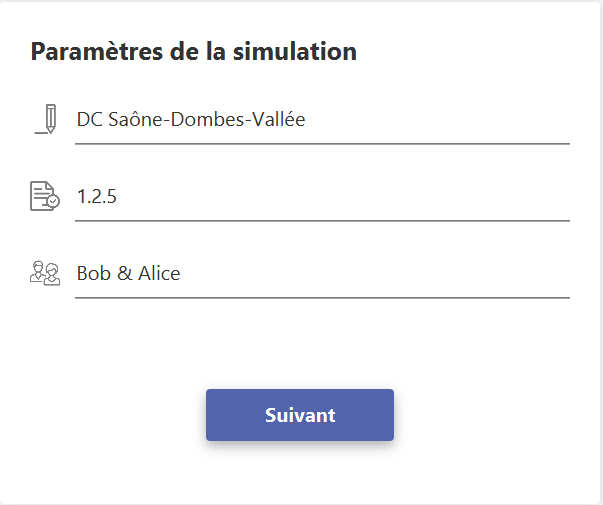
\includegraphics[height=6cm]{partie3/images/simulation.png}
		\caption{L'écran des paramètres de la simulation}
	\end{minipage}\hfill
	\begin{minipage}{0.48\textwidth}
		\centering
		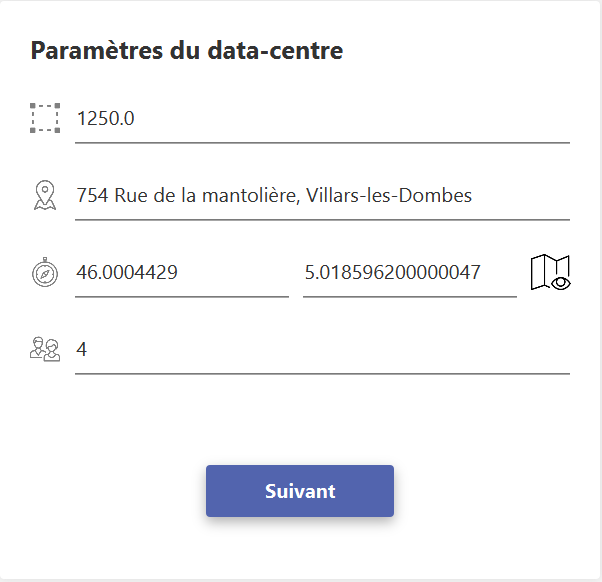
\includegraphics[height=6cm]{partie3/images/datacenter.png}
		\caption{L'écran des paramètres du centre de données}
	\end{minipage}\hfill
\end{figure}

\subsubsection{La géolocalisation}
Pour choisir l'adresse du centre de données, l'utilisateur a plusieurs choix. Il peut tout d'abord entrer une adresse qui sera automatiquement géocodée en coordonnées GPS. Il peut également entrer des coordonnées GPS qui seront automatiquement géocodées en une adresse. Il peut également choisir l'emplacement du centre de données en cliquant sur une carte.

\begin{figure}[h!]
	\begin{center}
		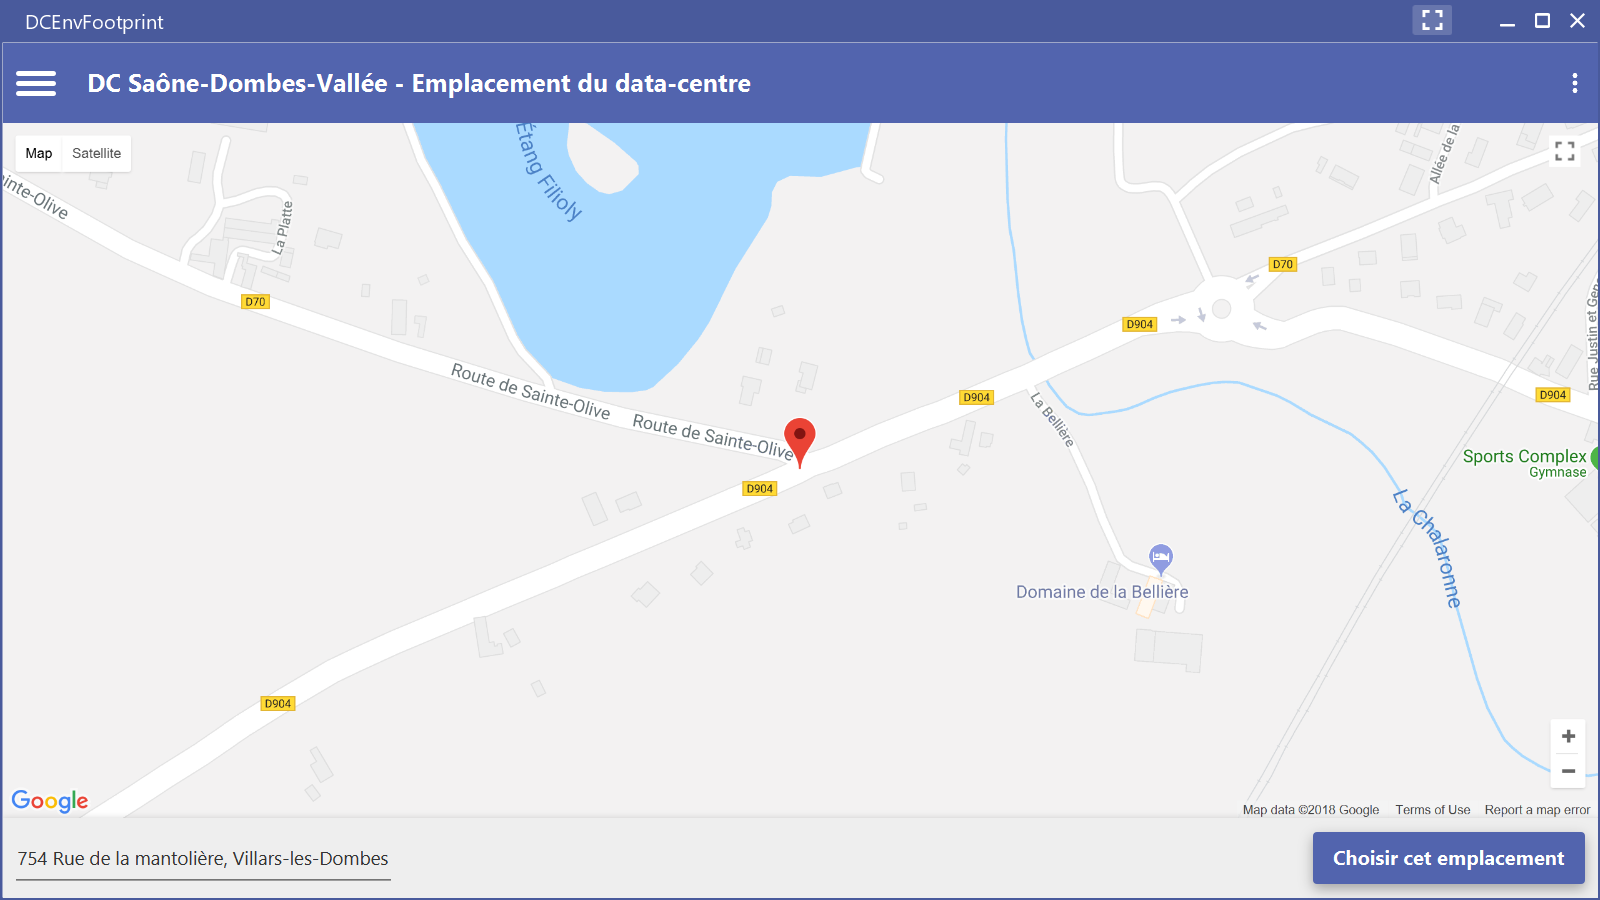
\includegraphics[scale=0.50]{partie3/images/carte.png}
		\caption{La carte permettant de choisir l'emplacement du centre de données}
	\end{center}
\end{figure}
\newpage
\subsubsection{La liste des périphériques de calcul}
L'utilisateur peut spécifier la liste des périphériques de calcul utilisés dans le centre de données. Une autocompletion depuis la base de données est fournie ce qui permet de choisir le bon modèle si il est disponible dans la base données. Une fois sélectionné la consommation d'énergie est automatiquement ajoutée.

\begin{figure}[h!]
	\begin{center}
		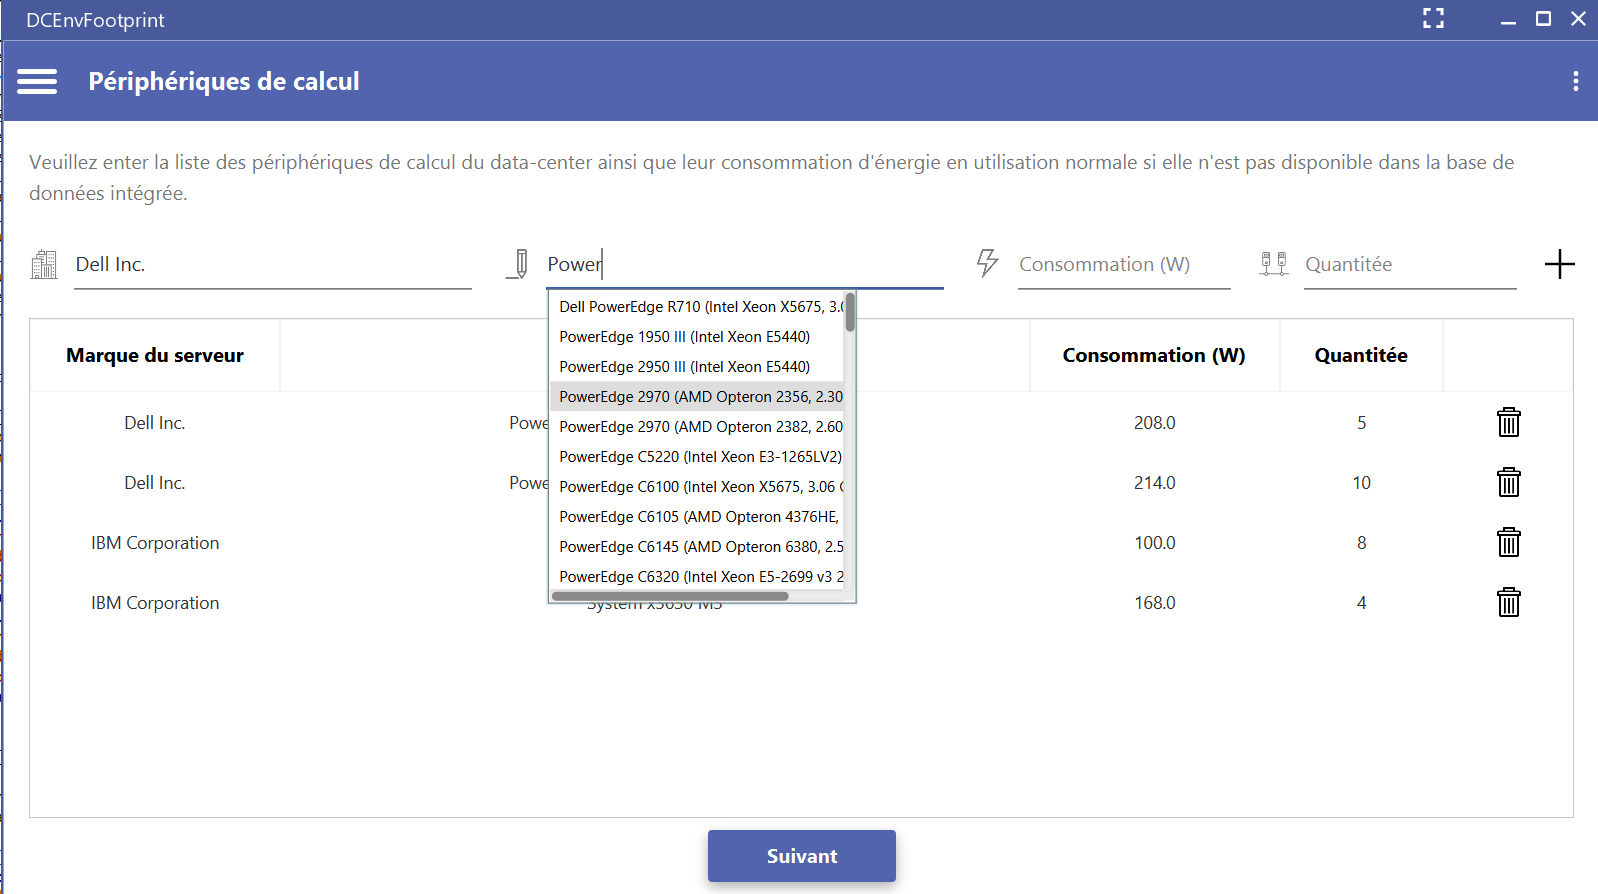
\includegraphics[scale=0.4]{partie3/images/calculation.png}
		\caption{L'écran permettant de saisir la liste des périphériques de calcul}
	\end{center}
\end{figure}

Il peut ensuite modifier n'importe quel modèle en cliquant sur les cellules du tableau. Il peut également supprimer un périphérique grâce au bouton sur la droite.

\subsubsection{La saisie des autres périphériques}
L'utilisateur peut également saisir les périphériques de stockage et les périphériques réseaux dans des écrans similaires à l'écran de saisie des périphériques de calcul. Cependant comme il n'existe pas de base de données pour ces équipements, il n'y a pas d'autocompletion. L'utilisateur devra se référer au manuel constructeur afin de définir la consommation d'énergie de son matériel.

\subsubsection{La gestion de la chaleur}
A partir des données entrées, le simulateur calcule automatiquement la dissipation de chaleur dans le centre de données. La méthode de calcul est basé sur un livre blanc de APC, une filière de Schneider Electric.\\
Pour répondre a cette quantité de chaleur, l'utilisateur peut choisir différentes formes de refroidissement dans la liste déroulante et les combiner. Comme certaines sources de refroidissement consomment de l'énergie, on laisse à l'utilisateur la possibilité de l'indiquer.

\begin{figure}[h!]
	\begin{center}
		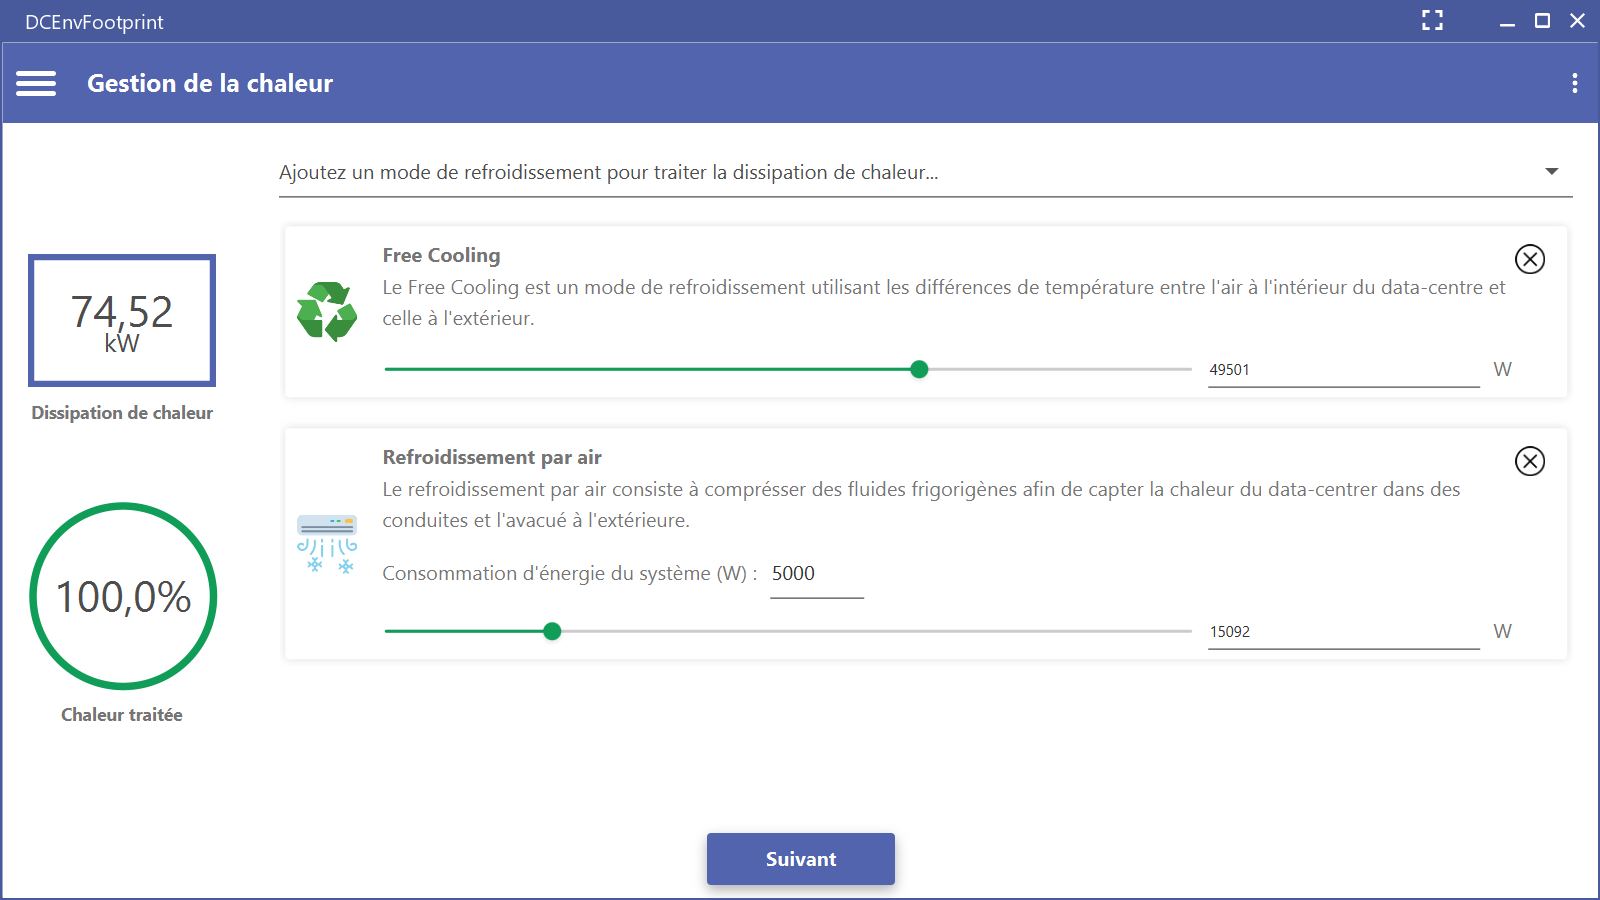
\includegraphics[scale=0.5]{partie3/images/chaleur.png}
		\caption{L'écran permettant de choisir les méthode de refroidissement}
	\end{center}
\end{figure}

\subsubsection{La réutilisation de chaleur}
Si le centre de données réutilise une partie de la chaleur créée par l'équipement informatique, l'utilisateur peut l'indiquer dans un écran dédié. Il peut également indiquer la quantité d'énergie utilisé pour ce retraitement de la chaleur. Cette information est importante car elle est prise en compte par certains indicateurs.

\subsubsection{La saisie des sources d'énergie}
Le simulateur calcule automatiquement la quantité d'électricité nécessaire au fonctionnement du centre de données. Il se base encore une fois sur un livre blanc d'APC.\\
Pour répondre à cette demande l'utilisateur peut ajouter des sources d'énergies depuis la liste déroulante et indiquer la quantité d'électricité qu'elle produit. Cet écran prend en compte l'énergie qui peut être produite sur site, comme vous pouvez le voir dans la capture d'écran suivante.

\begin{figure}[h!]
	\begin{center}
		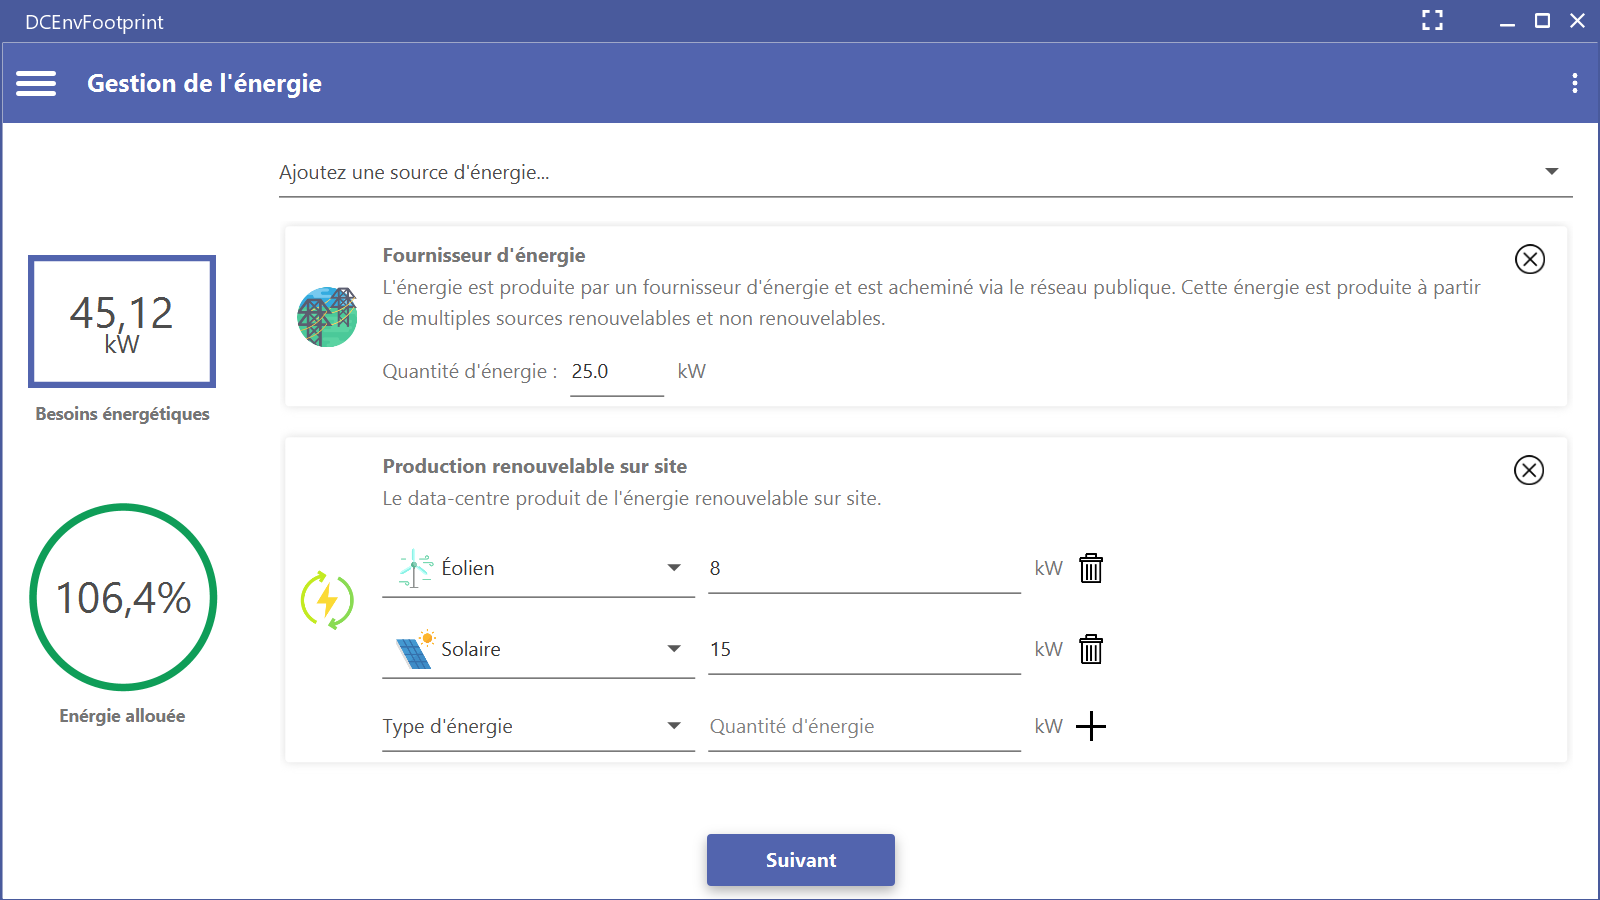
\includegraphics[scale=0.5]{partie3/images/energie.png}
		\caption{L'écran permettant de choisir les sources d'énergie}
	\end{center}
\end{figure}

\subsubsection{La vérification des champs}
Évidemment tous les champs modifiables par l'utilisateur sont vérifiés automatiquement et en temps réel afin qu'il ne mettent pas la simulation dans un état incohérent. L'utilisateur ne peut pas sauvegarder sa simulation ou passer à l'écran suivant si les champs contiennent des erreurs. Si il y a des erreurs lors de la sauvegarde, l'utilisateur est envoyé sur l'écran qui pose problème où les erreurs sont mis en évidences.

\begin{figure}[h!]
	\begin{center}
		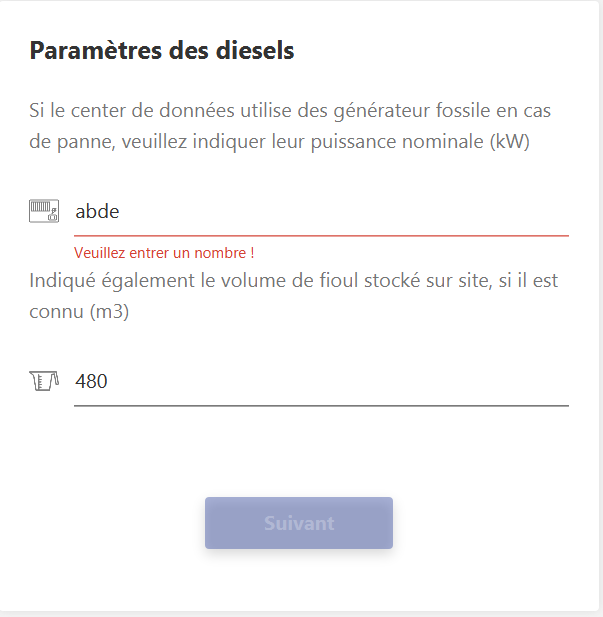
\includegraphics[scale=0.6]{partie3/images/verif.png}
		\caption{La gestion d'une erreur dans un champs}
	\end{center}
\end{figure}
\newpage
\subsubsection{La génération de rapport}
Une fois que l'utilisateur a entrer tous les paramètres dont le simulateur à besoin un rapport est généré automatiquement. Il calcule automatiquement les indicateurs et détaille le calcul de certains. Cependant il est loin d'être parfais, une  partie des indicateurs ne sont pas détaillés par faute de temps. Il aurait également été intéressant d'intégrer les sources systématiquement dans le raport. On remarque aussi que des commentaires utilisateurs ont été prévu, mais non implémentés.

Vous retrouverez en \hyperref[appendix:report]{Annexe C} un exemple de rapport généré par le simulateur.